\documentclass[a4paper,12pt]{article}
\RequirePackage[l2tabu, orthodox]{nag}
\usepackage{setspace}
\usepackage{amsfonts}
\usepackage{amsmath}
\usepackage{graphicx}
%Enable fr support
\usepackage[utf8]{inputenc} 
\usepackage[T1]{fontenc} 
\usepackage{lmodern} % load a font with all the characters

%Assign document variables
\date{\today}
\title{Projet Final;}
\author{tmp}
\newcommand{\Author}{Kevin Belisle}
\newcommand{\Authorr}{Michael Leblanc}
\newcommand{\Authorrr}{Temp}
\newcommand{\Teacher}{Michel Boyer}
\newcommand{\ClassNum}{IFT-2935}
\newcommand{\ClassName}{Bases de données}
\newcommand{\DateMMMMYYYY}{Mai 2018}
\newcommand{\tab}[1]{\hspace{.05\textwidth}\rlap{#1}}
\makeatletter
%Custom Header & Footer
\usepackage{fancyhdr}
\pagestyle{fancy}
\fancyhf{}
\fancyhead[L]{\@title}
\fancyhead[R]{\thepage}
\fancyfoot[L]{Kevin Belisle \& Michael Leblanc \& Temp}
\fancyfoot[R]{\DateMMMMYYYY}
\renewcommand{\footrulewidth}{0.4pt}% default is 0pt

\begin{document}
	\begin{titlepage} 
		\begin{center}
			\textsc{\normalsize Université de Montréal}\\[2.25cm]
			 
			\textsc{\LARGE \@title}\\[2.25cm]
			
			\textsc{\small Par}\\[0.25cm]
			\textsc{\LARGE \Author}\\[0.25cm]
			\textsc{\normalsize (20018469)}\\[0.25cm]
			\textsc{\LARGE \Authorr}\\[0.25cm]
			\textsc{\normalsize (20005779)}\\[0.25cm]
			\textsc{\LARGE \Authorrr}\\[0.25cm]
			\textsc{\normalsize (00000000)}\\[2cm]
			
			\textsc{\normalsize Baccalauréat en informatique}\\
			\textsc{\normalsize Faculté des arts et des sciences}\\[2.25cm]
			
			\textsc{\small Travail présenté à \Teacher}\\
			\textsc{\small Dans le cadre du cours \ClassNum}\\
			\textsc{\small \ClassName}\\[2.25cm]
			
			\textsc{\normalsize \DateMMMMYYYY}\\[1.5cm]
		\end{center}
	\end{titlepage}
	\begin{spacing}{1}
	%La représentation E-A de la base relationnelle accompagné d'explications%
	\section*{Modèle entité-association}
	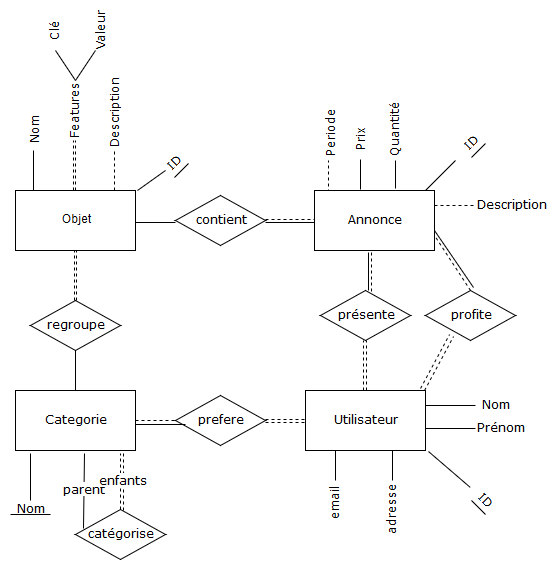
\includegraphics[scale=0.6]{modeleEA.png}
	\subsection*{Catégorie}
	TODO
	\subsection*{Objet}
	TODO
	\subsection*{Annonce}
	TODO
	\subsection*{Utilisateur}
	TODO
	%Le schéma relationnel de la base%
	\section*{Schéma relationnel}
	Utilisateur(\underline{iduser}, prenom, nom, email, adresse)\\
	Categorie(\underline{ncat},\#pcat)\\
	Prefere(\underline{\#iduser},\underline{\#ncat})\\
	Objet(\underline{idobj}, name, ncat, odesc)\\
	Feature(\underline{\#idobj},\underline{fname},fvalue)\\
	Annonce(\underline{idannonce},\#idobj,\#idvendeur,datedebut,datefin,prix,qte,description)\\
	Partage(\underline{\#idacheteur},\underline{\#idannonce},\underline{data})
	% PK %
	% Formats standard %
	% Separe ou duplication %
	% Choix d'implementation %
	\section*{Explication du DDL}
	\subsection*{Catégorie}
	Nous avons choisi le nom de la catégorie (ncat) comme clé primaire puisque c'est le seul et unique champ propre à la table. Le champs pcat réfère à la catégorie parent (NULL si aucun parent) ainsi il est possible de trouver tous les objets faisant partie de la catégorie choisie et de ces enfants.
	\subsection*{Objet}
	TODO
	\subsection*{Annonce}
	TODO
	\subsection*{Utilisateur}
	TODO
	% L'ensemble des requêtes en SQL et explication du résultat attendu %
	\section*{Requêtes SQL}
	\subsection*{Vues}
	
	\begin{verbatim}
	    CREATE VIEW projet.annonce_actif AS
            SELECT a.*, a.qte - COUNT(p.idannonce) as "qteleft"
            FROM projet.annonce as "a"
            LEFT JOIN projet.partage as "p" 
                ON a.idannonce = p.idannonce
            WHERE (datefin IS NULL OR now() < a.datefin)
            GROUP BY (a.idannonce)
            HAVING COUNT(p.idannonce) < a.qte;

	\end{verbatim}
	Créer une vue qui contient toutes les annonces qui sont présentement actives, c'est-à-dire les annonces dont la date de fin n'est pas atteinte et dont la quantité n'est pas encore zéro.
	
	\subsection*{SELECT}
	
	\begin{verbatim}
	    SELECT * FROM projet.utilisateur;
	\end{verbatim}
	Sélectionne toutes les colonnes et les occurrences de la table utilisateur.
	
	\begin{verbatim}
	    SELECT
    	    o.name AS objet_nom,
    	    o.ncat AS objet_categorie,
    	    p.date AS partage_date,
    	    a.prix,
    	    u.prenom AS acheteur_prenom,
    	    u.nom AS acheteur_nom,
    	    v.prenom AS vendeur_prenom,
    	    v.nom AS vendeur_nom
	    FROM
        	projet.annonce AS "a"
        	INNER JOIN projet.partage AS "p"
        	    ON a.idvendeur = \$1 AND a.idannonce = p.idannonce
        	NATURAL JOIN projet.objet AS "o"
        	INNER JOIN projet.utilisateur AS "u"
        	    ON u.iduser = p.idacheteur
        	INNER JOIN projet.utilisateur AS "v"
        	    ON v.iduser = a.idvendeur ORDER BY date ASC;
    \end{verbatim}
Sélectionne les colonnes objet.name, objet.ncat, partage.date, annonce.prix, utilisateur.prenom, utilisateur.nom, utilisateur.prenom et utilisateur.nom (renommées respectivement objet\_nom, objet\_categorie, partage\_date, prix, acheteur\_prenom, acheteur\_nom, vendeur\_prenom, vendeur\_nom) de la table résultant de la jointure des tables annonces, partage, objet et utilisateur en spécifiant l'ID de la personne profitant d'un partage (ou vente).
Cette requête sert à obtenir une table dont chaque ligne correspond à une annonce dont une personne \$1 a profitée.

    \begin{verbatim}
    SELECT
        o.name AS objet_nom
        o.ncat AS objet_categorie
        p.date AS partage_date
        a.prix
        u.prenom AS vendeur_prenom
        u.nom AS vendeur_nom
        ac.prenom AS acheteur_prenom
        ac.nom AS acheteur_nom
    FROM
        projet.partage AS "p"
        INNER JOIN projet.annonce AS "a"
            ON p.idacheteur = 1 AND a.idannonce = p.idannonce
            NATURAL JOIN projet.objet AS "o"
        INNER JOIN projet.utilisateur AS "u"
            ON u.iduser = a.idvendeur 
        INNER JOIN projet.utilisateur AS "ac"
            ON ac.iduser = p.idacheteur;
	\end{verbatim}
Sélectionne les colonnes objet.name, objet.ncat, partage.date, annonce.prix, utilisateur.prenom, utilisateur.nom, utilisateur.prenom et utilisateur.nom (renommées respectivement objet\_nom, objet\_categorie, partage\_date, prix, acheteur\_prenom, acheteur\_nom, vendeur\_prenom, vendeur\_nom) de la table résultant de la jointure des tables annonces, partage, objet et utilisateur en spécifiant l'ID de la personne ayant mit en ligne l'annonce.
Cette requête sert à obtenir une table dont chaque ligne correspond à une annonce mise en ligne par une personne \$1 et dont au moins une personne a pu profiter.

    \begin{verbatim}
    SELECT
	    fname AS feature_nom,
	    fvalue AS feature_valeur
    FROM projet.feature WHERE idobj = $1;
    \end{verbatim}
Sélectionne les colonnes feature.fname et feature.fvalue de la table feature et ses occurences où la valeur de la colonne feature.idobj vaut \$1.

    \begin{verbatim}
    SELECT
        aa.idannonce AS annonce_id
        aa.idobj AS objet_id
        aa.datedebut AS date_debut
        aa.datefin AS date_fin
        aa.prix
        aa.qte
        o.name AS objet_nom
        o.ncat AS objet_categorie
        o.odesc AS objet_description 
        u.prenom AS vendeur_prenom
        u.nom AS vendeur_nom
        u.email AS vendeur_email
        u.adresse AS vendeur_adresse
    FROM
        projet.annonce_actif AS "aa"
        INNER JOIN projet.objet AS "o"
            ON aa.idannonce = $1 AND aa.idobj = o.idobj
        INNER JOIN projet.utilisateur AS "u"
            ON aa.idvendeur = u.iduser;
	
	\end{verbatim}
Sélectionne les colonnes annonce\_actif.idannonce, annonce\_actif.idobj, annonce\_actif.datedebut, annonce\_actif.datefin, annonce\_actif.prix, annonce\_actif.qte, objet.name, objet.ncat, objet.odesc, utilisateur.prenom, utilisateur.nom, utilisateur.email, utilisateur,adresse (renommées respectivement annonce\_id, objet\_id, date\_debut, date\_fin, prix, qte, objet\_nom, objet\_categorie, objet\_description, vendeur\_prenom, vendeur\_nom, vendeur\_email, vendeur\_adresse) de la table résultant de la vue annonce\_actif et des tables objet et utilisateur en spécifiant l'ID de l'annonce.
Cette requête sert à obtenir les informations nécessaires en lien avec une annonce qui est toujours active.

    \begin{verbatim}
        SELECT * FROM projet.annonce_actif ORDER BY idannonce ASC        
    \end{verbatim}
Sélectionne toutes les colonnes de la table annonce\_actif et toutes ses occurences en les ordonnant par l'ID de l'annonce de façon croissante.

    \begin{verbatim}
        SELECT ncat,pcat,niveau FROM projet.categorie_listing
    \end{verbatim}
Sélectionne les colonnes ncat,pcat et niveau de la table categorie\_listing et toutes ses occurences.

    \begin{verbatim}
        SELECT * FROM projet.objet WHERE idobj = $1
    \end{verbatim}
Sélectionne toutes les colonnes de la table objet et toutes ses occurences dont l'ID de l'objet vaut \$1.

    \subsection*{INSERT}
    
    \begin{verbatim}
        INSERT INTO projet.partage (idacheteur, idannonce, date) VALUES($1,$2,now());
    \end{verbatim}
    Ajoute un nouveau partage dans la base de données avec une date de partage générée au moment de l'insertion.
    
    \begin{verbatim}
        INSERT INTO projet.utilisateur (prenom, nom, email, adresse) VALUES($1,$2,$3,$4);
    \end{verbatim}
    Ajoute un nouvel utilisateur dans la table utilisateur. Le ID de l'utilisateur est généré automatiquement par la base de données. 

    \begin{verbatim}
        INSERT INTO projet.prefere (iduser,ncat) VALUES($1,$2);
    \end{verbatim}
    Ajoute une nouvelle préférence d'un utilisateur dans la table prefere.
    
    \begin{verbatim}
        INSERT INTO projet.objet (name, ncat, odesc) VALUES($1,$2,$3);
    \end{verbatim}
    Ajoute un nouvel objet dans la table objet. Le ID de l'objet est généré automatiquement par la base de données.
    
    \begin{verbatim}
        INSERT INTO projet.annonce (datefin, prix, qte, idvendeur, idobj) VALUES ($1,$2,$3,$4,$5);
    \end{verbatim}
    Ajoute une nouvelle annonce dans la table annonce. Le ID de l'annonce est généré automatiquement par la base de données.


	\subsection*{DML}
	
	TODO
	% Captures d’écran de l’application avec description de fonctionnement de l’application%
	\section*{Guide Utilisateur}
	\subsection*{Historique des achats}
	\includegraphics[scale=0.6]{historique\_achats.png}
Il suffit de sélectionner un utilisateur et de cliquer sur le bouton rechercher pour obtenir une liste des achats effectuées par cet utilisateur. Par exemple, vous pouvez sélectionner l'utilisateur ``Sadlq Bahar'' avec l'ID 8.
    \subsection*{Historique des ventes}
    \includegraphics[scale=0.6]{historique\_ventes.png}
Il suffit de sélectionner un utilisateur et de cliquer sur le bouton rechercher pour obtenir une liste des ventes effectuées par cet utilisateur. Par exemple, vous pouvez sélectionner l'utilisateur ``Leon Dietrich'' avec l'ID 1.
    \subsection*{Ajout d'annonce}
    \includegraphics[scale=0.6]{ajout\_annonce.png}
Il faut tout d'abord sélectionner un utilisateur qui représentera l'annonceur (ou vendeur)
Les champs ``ID du vendeur'', ``Nom de l'objet'', ``Catégorie de l'objet'', ``Quantité d'objet'' et  ``Prix'' sont requis.
La quantité de l'objet doit être supérieur à 0 alors que le prix, lui, doit être supérieur ou égal à 0.
Les autres champs sont factulatifs. Si jamais on entre incorrectement des valeurs dans les champs requis, un message d'erreur s'affiche.

    \subsection*{Ajout d'utilisateur}
    \includegraphics[scale=0.6]{ajout\_utilisateur.png}
Tous les champs sont requis, sauf pour adresse et préférence. Si jamais on entre incorrectement des valeurs dans les champs requis, un message d'erreur s'affiche.

    \subsection*{Annonce}
    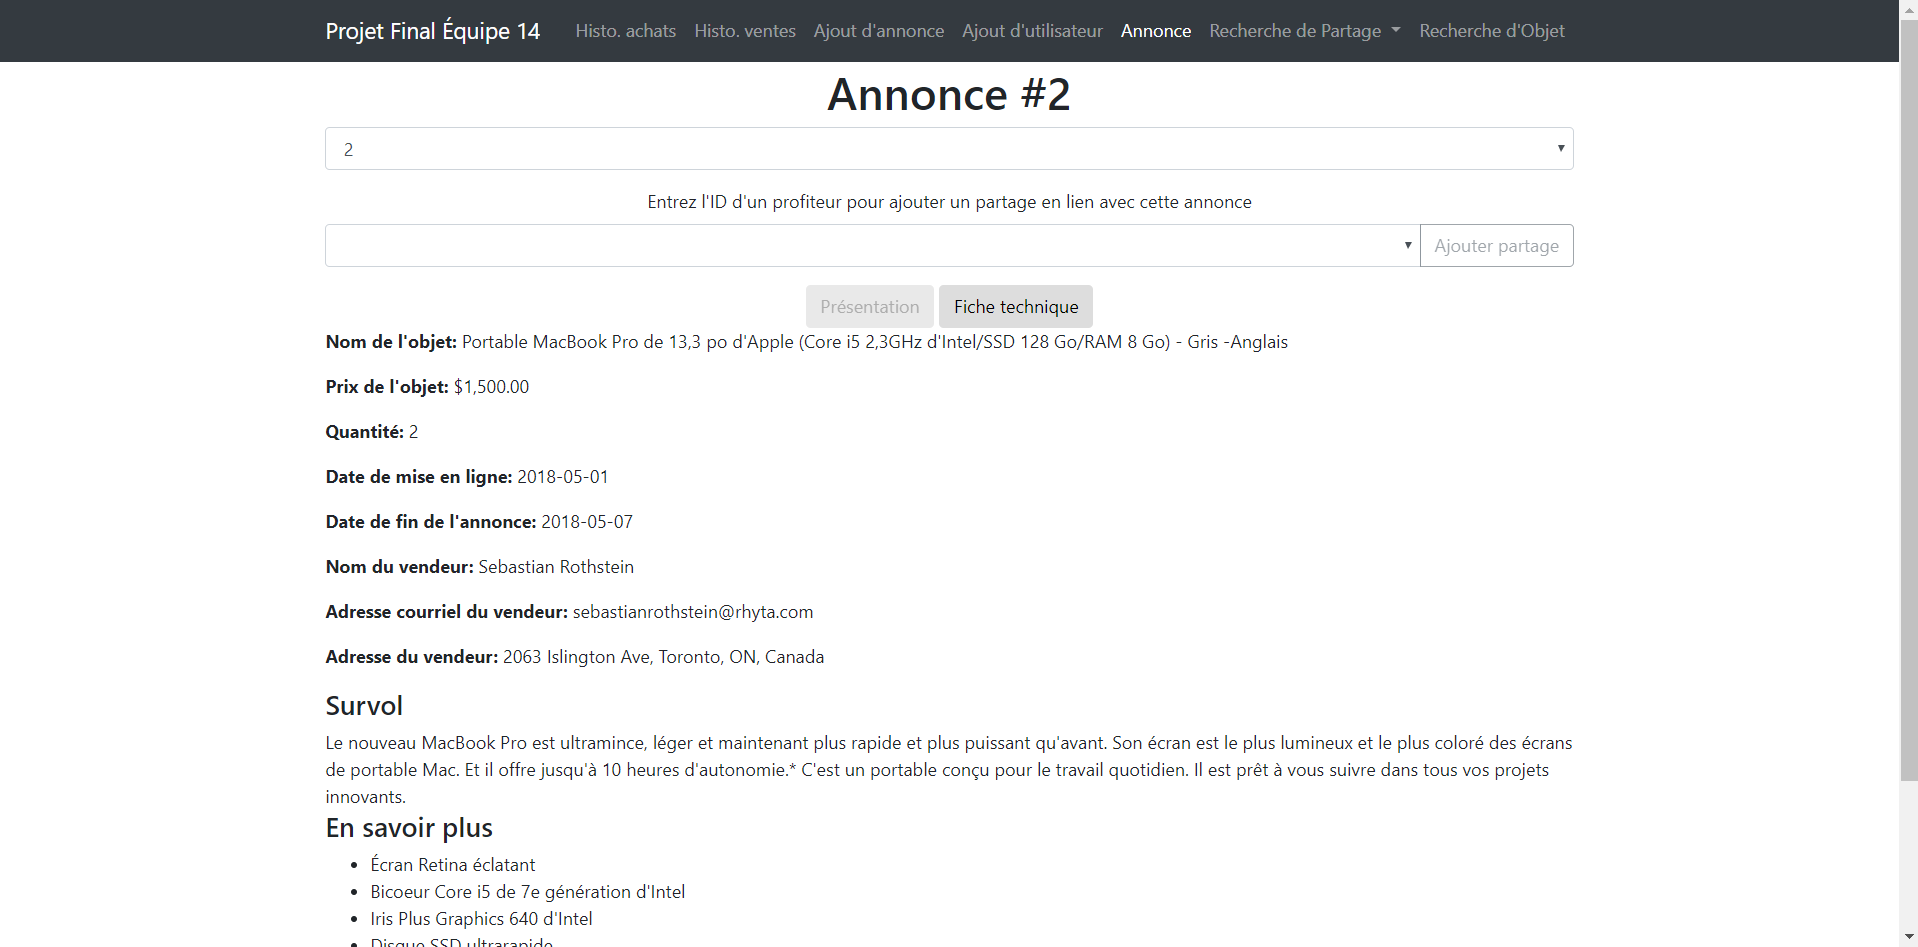
\includegraphics[scale=0.6]{annonce.png}
Tout d'abord, il faut choisir l'ID d'une annonce active. Le champ situé en dessous du titre contient toutes les annonces qui sont actives, donc on ne peut pas se tromper. Une fois l'annonce sélectionné, les informations la concernant sont affichées. Il est possible de naviguer entre la fiche technique de l'objet et la présentation de l'annonce en cliquant sur les boutons appropriés.	
Dans cette page, on peut aussi simuler un partage en sélectionnant d'un profiteur dans le champ au dessus des boutons ``Présentation'' et ``Fiche technique'' et en cliquant sur le bouton ajouter partage ensuite. Si tout s'est bien passé, un message de confirmation devrait apparaître.

    \subsection*{Recherche d'objet}
    \includegraphics[scale=0.6]{recherche\_objet.png}
Cette page sert à chercher la description d'un objet. Il suffit de cliquer sur ``Filtre'' pour voir s'afficher deux champs. Le premier correspond à la catégorie de l'objet en question. Le deuxième champ, facultatif permet de faire une recherche par nom de l'objet. Après avoir cliqué sur ``Appliquer'', une liste des objets trouvées devrait apparaître. On peut ensuite cliquer sur un des objets trouvés pour voir sa description. 
Par exemple, vous pouvez mettre comme catégorie ``Électronique'' et faire une recherche par nom avec le mot clé ``Intel''.

    \subsection*{Recherche de partage}
    TODO


	\end{spacing}                                                 
\end{document} 